%
% This is the LaTeX template file for lecture notes for CS267,
% Applications of Parallel Computing.  When preparing 
% LaTeX notes for this class, please use this template.
%
% To familiarize yourself with this template, the body contains
% some examples of its use.  Look them over.  Then you can
% run LaTeX on this file.  After you have LaTeXed this file then
% you can look over the result either by printing it out with
% dvips or using xdvi.
%

\documentclass{article}
%% \setlength{\oddsidemargin}{-0.25 in}
%% %% \setlength{\evensidemargin}{-0.25 in}
%% \setlength{\topmargin}{-0.6 in}
%% \setlength{\textwidth}{6.5 in}
%% \setlength{\textheight}{8.5 in}
\usepackage[margin=1in]{geometry}
\setlength{\headsep}{0.75 in}
\setlength{\parindent}{0 in}
\setlength{\parskip}{0.1 in}

%
% ADD PACKAGES here:
%

\usepackage{amsmath,amsfonts,graphicx}
\usepackage{algorithm,algorithmic,color}

%
% The following commands set up the lecnum (lecture number)
% counter and make various numbering schemes work relative
% to the lecture number.
%
\newcounter{lecnum}
\renewcommand{\thepage}{\thelecnum-\arabic{page}}
\renewcommand{\thesection}{\thelecnum.\arabic{section}}
\renewcommand{\theequation}{\thelecnum.\arabic{equation}}
\renewcommand{\thefigure}{\thelecnum.\arabic{figure}}
\renewcommand{\thetable}{\thelecnum.\arabic{table}}

%
% The following macro is used to generate the header.
%
\newcommand{\lecture}[4]{
   \pagestyle{myheadings}
   \thispagestyle{plain}
   \newpage
   \setcounter{lecnum}{#1}
   \setcounter{page}{1}
   \noindent
   \begin{center}
   \framebox{
      \vbox{\vspace{2mm}
    \hbox to 6.28in { {\bf Linear Algebra
                        \hfill Spring 2023} }
       \vspace{4mm}
       \hbox to 6.28in { {\Large \hfill Lecture #1: #2  \hfill} }
       \vspace{2mm}
       \hbox to 6.28in { {\it Lecturer: #3 \hfill Scribes: #4} }
      \vspace{2mm}}
   }
   \end{center}
   \markboth{Lecture #1: #2}{Lecture #1: #2}
   {\bf Note}: {\it LaTeX template courtesy of UC Berkeley EECS dept.}

   {\bf Disclaimer}: {\it These notes are based on the freely available online lectures by Prof. Gilbert Strang.
}

   \vspace*{4mm}
}

%
% Convention for citations is authors' initials followed by the year.
% For example, to cite a paper by Leighton and Maggs you would type
% \cite{LM89}, and to cite a paper by Strassen you would type \cite{S69}.
% (To avoid bibliography problems, for now we redefine the \cite command.)
% Also commands that create a suitable format for the reference list.
\renewcommand{\cite}[1]{[#1]}
\def\beginrefs{\begin{list}%
        {[\arabic{equation}]}{\usecounter{equation}
         \setlength{\leftmargin}{2.0truecm}\setlength{\labelsep}{0.4truecm}%
         \setlength{\labelwidth}{1.6truecm}}}
\def\endrefs{\end{list}}
\def\bibentry#1{\item[\hbox{[#1]}]}

%Use this command for a figure; it puts a figure in wherever you want it.
%usage: \fig{NUMBER}{SPACE-IN-INCHES}{CAPTION}
\newcommand{\fig}[3]{
			\vspace{#2}
			\begin{center}
			Figure \thelecnum.#1:~#3
			\end{center}
	}

 
% Use these for theorems, lemmas, proofs, etc.
\newtheorem{theorem}{Theorem}[lecnum]
\newtheorem{lemma}[theorem]{Lemma}
\newtheorem{proposition}[theorem]{Proposition}
\newtheorem{claim}[theorem]{Claim}
\newtheorem{corollary}[theorem]{Corollary}
\newtheorem{definition}[theorem]{Definition}
\newenvironment{proof}{{\bf Proof:}}{\hfill\rule{2mm}{2mm}}

% **** IF YOU WANT TO DEFINE ADDITIONAL MACROS FOR YOURSELF, PUT THEM HERE:

\begin{document}

%FILL IN THE RIGHT INFO.
%\lecture{**LECTURE-NUMBER**}{**DATE**}{**LECTURER**}{**SCRIBE**}
\lecture{1}{The Geometry of Linear Equations
}{Prof. Gilbert Strang}{Chanho Jung}
%\footnotetext{These notes are partially based on those of Nigel Mansell.}

% **** YOUR NOTES GO HERE:

% Some general latex examples and examples making use of the
% macros follow.  
%**** IN GENERAL, BE BRIEF. LONG SCRIBE NOTES, NO MATTER HOW WELL WRITTEN,
%**** ARE NEVER READ BY ANYBODY.

\section{Linear Equations}

The fundamental problem of linear algebra is to solve n linear equations in n.
unknowns.


\begin{center}
$2x-y=0$

$-x+2y=3$


$\begin{bmatrix}
2 & -1 \\
-1 & 2 
\end{bmatrix}
\begin{bmatrix}
x\\
y
\end{bmatrix}$
$=
\begin{bmatrix}
0\\
3
\end{bmatrix}$

$A\textbf{x}=\textbf{b}$
\end{center}

The linear equations are Ax=b and the idea now is to solve this particular example,and then step back to see the bigger picture.


\subsection{Row picture}
Plot \textbf{all the points} that satisfy that equations.
\begin{center}
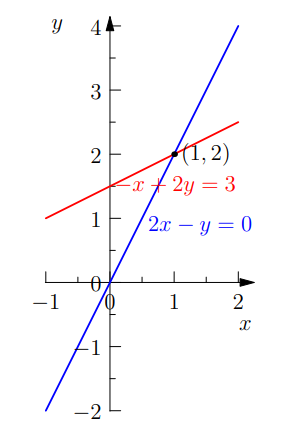
\includegraphics{images/rowpicture.png}
    
\end{center}

(1,2) is the all-important point that lies on both lines. because this solves both equations. Seeing the row picture, first of all, for n=2, two equations and two unknowns.

\subsection{Column picture}
Look at the columns of the matrix.
\begin{center}
$x$
$\begin{bmatrix}
2  \\
-1  
\end{bmatrix}
$+ y$
\begin{bmatrix}
-1\\
2
\end{bmatrix}$
$=
\begin{bmatrix}
0\\
3
\end{bmatrix}$

\end{center}

and now what is the equation asking for?
It's asking us to find somehow to combine that vector. 

It's asking us to find the right \textbf{linear combination}.And it's the most fundamental operation in the whole course.

Multiply by some numbers and add. That's a linear combination. This is Algebra. Then what's the geometry(what's the picture that goes with it)?
\begin{center}
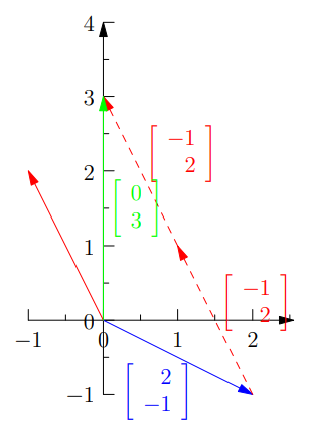
\includegraphics{images/colpicture.png}
    
\end{center}

\begin{center}
$1$
$\begin{bmatrix}
2  \\
-1  
\end{bmatrix}
$+ 2$
\begin{bmatrix}
-1\\
2
\end{bmatrix}$
$=
\begin{bmatrix}
0\\
3
\end{bmatrix}$

\end{center}
Combine first column vector and second column vector to get vector \textbf{b}.

\textbf{Then, what are all the combinations?} If I took all the \textbf{x} and all the \textbf{y}, all the combinations, What would be all the results? The results would be that I could get any right-hand side at all.
\subsection{Extend dimension}
Let's do 3x3

\begin{align*} 
2x - y &=  0 \\ 
-x + 2y -z&=  -1\\
-3y+4z &=4
\end{align*}
\begin{center}
$\begin{bmatrix}
2 & -1 & 0\\
-1 & 2 & -1 \\
0 & -3 & 4
\end{bmatrix}
\begin{bmatrix}
x\\
y\\
z
\end{bmatrix}$
$=
\begin{bmatrix}
0\\
-1\\
4
\end{bmatrix}$  

$A\textbf{x}=\textbf{b}$
\end{center}

In this case, the points that satisfy all equations make a plane. Each row gives us a plane in three dimensions. those three things meet a point. The main point is that the three planes, because they're not parallel,they're not special. 

This row picture getting a little hard to see. When we look at three planes meeting,it's not clear and in four dimensions probably a little less clear.

\textbf{How about the column picture?}

\begin{center}
$x$
$\begin{bmatrix}
2  \\
-1  \\
0
\end{bmatrix}
$+ y$
\begin{bmatrix}
-1\\
2 \\
3
\end{bmatrix}$
$+ z$
$\begin{bmatrix}
0\\
-1 \\
4
\end{bmatrix}$
=
$\begin{bmatrix}
0\\
-1\\
4
\end{bmatrix}$

\end{center}
The left-side is a linear combination of three vectors, so we want to know what combination of those three vectors produces that one. If x=0,y=0,z=1 ,the combinations make \textbf{b}.
\subsection{Linear Independence}
It's the next lecture, which is about elimination, which is the systematic way that every body would solve the equations.


\textbf{Can I solve these equations for every right-hand side? that's the algebra question.}

\textbf{Can I solve Ax=b for every b?}

\textbf{Do the linear combinations of the columns fill three dimensional space?}

Every b means all the b in three dimensional space. Elimination will give me a way to find it.




For this matrix A, answer is YES. because I choose good matrix. non-singular matrix, An invertible matrix.

If these three columns all lie in the same plane, then their combinations will lie in that same plane.

It's can solve If b is in the same plane, but most b would be out of the plane and unreachable. So that would be a \textbf{singular} case. the matrix is not invertible. there would not be a solution for every b.

If I choose those columns so that they're not independent,


A times x when I multiply a matrix by a vector. It's multiply that Matrix times vector. then how do you multiply a matrix by a vector?

There is two way.

First is columns again!

\begin{center}


$A\textbf{x}=\textbf{b}$

$\begin{bmatrix}
2 & 5 \\
1 & 3 
\end{bmatrix}
\begin{bmatrix}
1\\
2
\end{bmatrix}$
$=?$


$\begin{bmatrix}
2 & 5 \\
1 & 3 
\end{bmatrix}
\begin{bmatrix}
1\\
2
\end{bmatrix}$
$= 1$
$\begin{bmatrix}
2 \\
1  
\end{bmatrix}
$+2$
\begin{bmatrix}
5\\
3
\end{bmatrix}$
$=$
$\begin{bmatrix}
12\\
7
\end{bmatrix}$

\end{center}

Second is the idea of a dot product. Do it by rows and each row times x that call a dot product. The point is Ax is a combination of the columns of A.
\end{document}





